% Pacotes e configurações padrão do estilo "article"\
% -------------------------------------
\documentclass[a4paper,11pt]{article}
% Layout
% --------------------------------------------------------------------------------
%     Gráficos e layout ----------------------------------------------------------------------

\ifx\pdfmatch\undefined
\else
    \usepackage[T1]{fontenc}
    \usepackage[utf8]{inputenc}
\fi
% xetex:
\ifx\XeTeXinterchartoks\undefined
\else
    \usepackage{fontspec}
    \defaultfontfeatures{Ligatures=TeX}
\fi
% luatex:
\ifx\directlua\undefined
\else
    \usepackage{fontspec}
\fi
% End engine-specific settings

%      Fonte --------------------------------------------------------------------------------
%\usepackage{lmodern}
\usepackage{times}
%     Pacotes adicionados -------------------------------------------------------------------
\usepackage{ae}
%     Língua e hifenização ------------------------------------------------------------------
\usepackage[portuguese]{babel}
\usepackage{hyphenat}
%      Outros --------------------------------------------------------------------------------
\usepackage{fancyhdr}
\usepackage{sectsty}
\usepackage{float}
\usepackage{graphicx}
%\usepackage[pdftex]{color,graphicx}
\usepackage{hyperref}
\usepackage{enumerate} % Permite alterar Layout do enumerate
%\usepackage{pdflscape} % Permite alterar a orientação da pagina
%\usepackage{ifthen} % Permite usar condicionais ifelse
%\usepackage[table]{xcolor} % Permite alterar as cores das celulas de uma tabela
\usepackage{amsmath,amssymb} % Ambiente para uso de elementos matemáticos
\usepackage{caption}
\usepackage{subcaption} % permite o uso de multiplas figuras com legenda
\usepackage{minted} % FOrmatador para códigos de programas
\usepackage{natbib} % Para referencia bibliográfica
\usepackage{url} % pacote url
% Layout do documento ------------------------------------------------------------------------
%     Bordas e tamanho da página ------------------------------------------------------------
\usepackage{geometry} 
 \geometry{ % Padrõa ABNT para relatórios
 a4paper,
 left=30mm,
 right=20mm,
 top=30mm,
 bottom=20mm
 }
%     Cabeçalho e Rodapé ---------------------------------------------------------------
\pagestyle{fancy}
  \lhead{}
  \chead{}
  \rhead{}
  \lfoot{}
  \cfoot{}
  \rfoot{\thepage}
%     Númeração ------------------------------------------------------------------------
  \pagenumbering{arabic}
%     Retas do cabeçalho e rodapé ------------------------------------------------------
  \renewcommand{\headrulewidth}{0.5pt}
  \renewcommand{\footrulewidth}{0.5pt}
%     Tamanho da letra de seções e derivadas --------------------------------------------
  \sectionfont{\normalsize}
  \subsectionfont{\small}
%     Hiperlinks ------------------------------------------------------------------------
  \hypersetup{
                  colorlinks,
                  citecolor=black,
                  filecolor=black,
                  linkcolor=black,
                  urlcolor=black
                  }
%     Dados do título e autores --------------------------------------------------------------
%\title{\tituloRelatorio}
\author{Rafael Lima}
%     Definições do pdf ----------------------------------------------------------------------
\hypersetup{
    unicode=false,          % non-Latin characters in Acrobat’s bookmarks
    pdftoolbar=true,        % show Acrobat’s toolbar?
    pdfmenubar=true,        % show Acrobat’s menu?
    pdffitwindow=false,     % window fit to page when opened
    pdfstartview={FitH},    % fits the width of the page to the window    
    pdfauthor={Rafael Lima},     % author
    pdfnewwindow=true      % links in new window
}
%     Outros ----------------------------------------------------------------------------
      %\renewcommand{\thesection}{(\alph{section})} % muda o estilo de númeração das sections
      % alterando a formatação dos numeradores de lista de itens
      \renewcommand\theenumi{\arabic{enumi}}
      \renewcommand\labelenumi{(\textit{\theenumi})}
	  \renewcommand\theenumii{\arabic{enumii}}
	  \renewcommand\labelenumii{(\textit{\theenumi.\theenumii})}
      
% ---------------------------------------------------------------------------------------


\newcommand{\tituloRelatorio}{Relatório 2 - Fresa CNC}
\title{\tituloRelatorio}
\hypersetup{pdftitle={\tituloRelatorio}}% title
% Definições Auxiliares
% -----------------------------------------------------------------
%\input{relat_aux.tex}
% ----------------------------------~>ø<~---------------------------------------
\begin{document}
% Capa e Índice ---------------------------------------------------------------
%--------------------------------------------------- Capa --------------------------------------------
%\newpage
\begin{flushleft}
Universidade de Brasilia - UnB\\
Departamento de Engenharia Mecânica\\
Disciplina: Tecnologia de Comando Numérico\\
%Professor: 
\end{flushleft}

\vspace{0.3\textheight}
\begin{center}
    \Huge\textbf{\\\tituloRelatorio \\}
\end{center}

\vspace{\fill} % Manda o resto para o fundo da página

\begin{flushleft}
\textbf{Aluno:}\\
\vspace{2mm}
\begin{tabular}{ll}
    Rafael Lima & 10/0131093
\end{tabular}
\end{flushleft}

%\thispagestyle{empty} % Retira o cabeçalho e o rodapé da página

% ------------------------------------------------- Índice -------------------------------------------
%\newpage
%\tableofcontents
\newpage
% ----------------------------------------------------------------------------------------------------



% Conteudo -------------------------------------------------------------------

\section{Objetivos}

\begin{itemize}
    \item Estudo das Etapas de Fabricação para peças em uma Fresa de 3 eixos
    \item Avaliação de Capabilidade de Fresa CNC Educacional
\end{itemize}

\section{Introdução Teórica}
% Contextualização sobre fabricação de peças de geometria axial
% - Eixos, Pião
% Conceito básico de Usinagem

\subsection{Fresa}
% O que é um Torno
% Como Funciona
% Operações  
% Torno CNC


\subsubsection{Código G}
% Origem do Código G
% Funções Empregadas

\subsection{Fresa CNC Didática}
Neste trabalho será utilizado como maquinário um torno didático desenvolvido por Miguel para o laboratório GRACO da UnB.\cite{mgutierrez_2013}. A fresa é constituida de uma Furadeira Dreamel acomplada a uma torre sobre uma uma mesa de eixos movimentada por servo motores. O equipamento é controlado através do sistema \hyperref[sec:linuxCNC]{\textit{LinuxCNC}} por meio de instruções feitas em código G. Os comandos interpretados pelo LinuxCNC são convertidos em instruções para uma placa controladora acionando dos três motores de passo  que controlam a altura da furadeira e a posição da mesa no qual é posicionada a broca ser utilizada.

\begin{figure}[H]
    \centering
    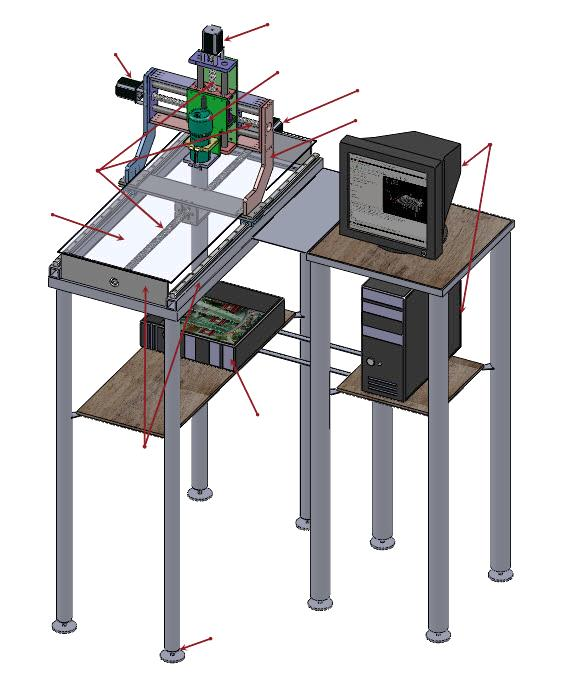
\includegraphics[width = 0.6\linewidth]{img/relat2/routerCNC}
    \caption{Simulação no Sistema CNC Web Simulator}
    \label{fig:vela-simCNCWebSimulator}
\end{figure}

%\subsection{Estudo de Capabilidade}
% Fontes de Erro de Medida
% Recomendações para evitar erros

\section{Fresamento}
 Será usinado uma placa de madeira compensado de $200x200\ mm^2$ de área com $15\ mm$ de espessura.

\subsection{Projeto da Peça}
O desenho original da peça foi inspirado na logo do Projeto Edubot da UnB. A partir do qual foram feitas as medidas relacionando as dimensões de cada parte de maneira relativa. Primeiramente a peça foi desenhada em papel milimetrado. Para o desenho foram exploradas 4 tipos de operações: desbaste de raio, corte reto com angulação em relação ao eixo de peça, sangramento, corte com interpolação circular. Desta forma poderiam ser feito a avaliação da precisão do torno em situações avaliando a movimentação.

\begin{figure}[H]
    \centering
    
\includegraphics[width = 0.6\linewidth]{img/relat2/edubot}
    \caption{Simulação no Sistema CNC Web Simulator}
    \label{fig:edubot}
\end{figure}

\subsection{Simulação}
\subsubsection{CNC Web Simulator}
A descrição em Código G foi avaliado utilizando o sistema CNC Web Simulator desenvolvido pelo Felipe Caixeta.\cite{filipecaixeta_2016} A escolha deste  simulador foi por este permitir uma rápida análise do efeito de cada instrução no desenho final da peça.

\begin{figure}[H]
    \centering
    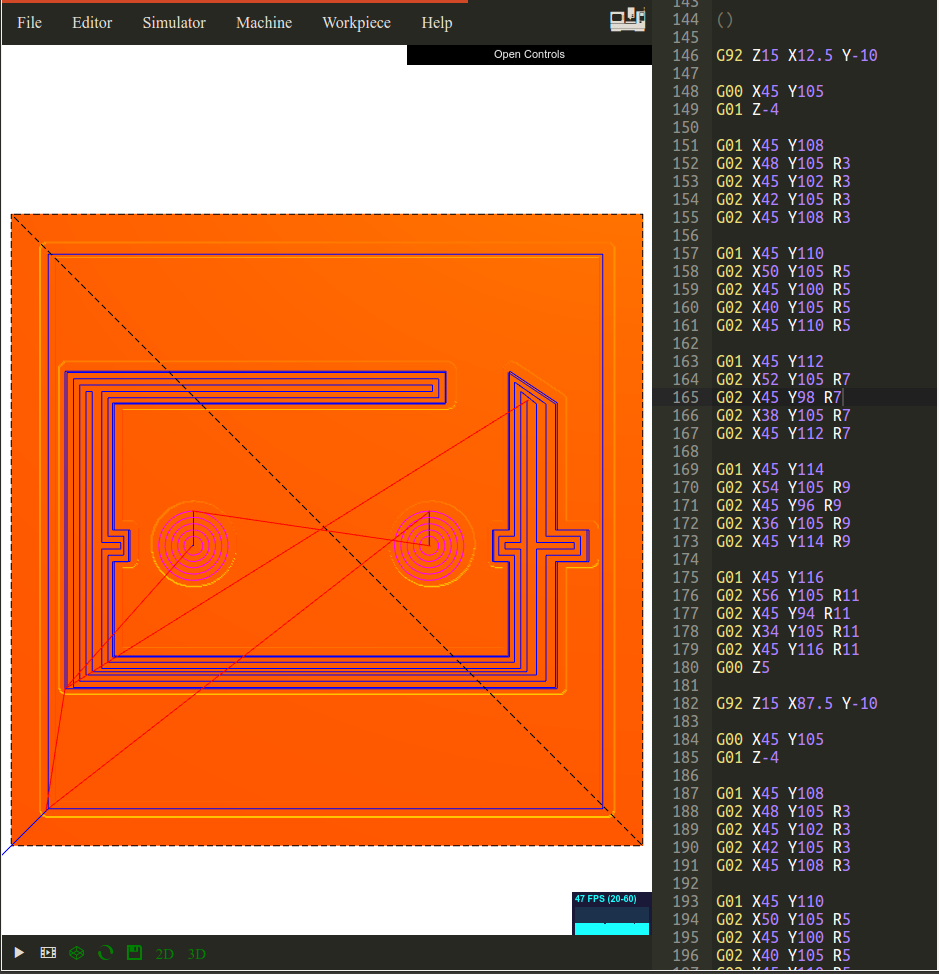
\includegraphics[width = 0.6\linewidth]{img/relat2/sim-fresa-web2}
    \caption{Simulação no Sistema CNC Web Simulator}
    \label{fig:placa-simCNCWebSimulator}
\end{figure}

\subsection{Fresamento}
Para a etapa de Fresamento foram modificadas todas movimentações em $G0$ para $G01$ no código G e removido as instruções $G92$ pois o torno conta com apenas uma velocidade e o zeramento é feito de maneira manual. Foi feito o seguinte procedimento para confecção do desenho na placa:
\begin{enumerate}
    \item Fixação da Vela na placa de madeira na mesa
    \item Upload do código na máquina de controle através de um pen drive
    \item Zeramento da posição da mesa através do posicionamento no eixo $Z$ da ponta da ferramenta à $12.5\ mm$ das bordas laterais da peça em relação a quina inferior esquerda com auxílio do sistema LinuxCNC.
    \item Acionamento do Furadeira através da chave de Liga/Desliga do equipamento.
    \item Início da execução programa da Peça atráves do LinuxCNC.
    \item Remoção do material com auxílio de uma aspirador de pó com a usinagem em andamento para acumulo de sujeira nas nos eixos da mesa.
    \item Desligamento do rotor através da chave de Liga/Desliga ao fim da usinagem.
    \item Remoção da vela da castanha.
\end{enumerate}

No entanto, houveram duas falhas no código G. Durante a operação de perfilamento o valor de Z estava errado e a broca apenas passou por cima da placa sem efetuar nenhum corte e o segundo erro foi a existência da instrução $G92$ que provocou um furo na profundidade errada e a execução do código teve de ser interrompida no meio. Em decorrência de tais fatos, o desenho final não pode ser concluído como pode ser conferido na figura \ref{fig:placa-final}.

\begin{figure}[H]
    \centering
    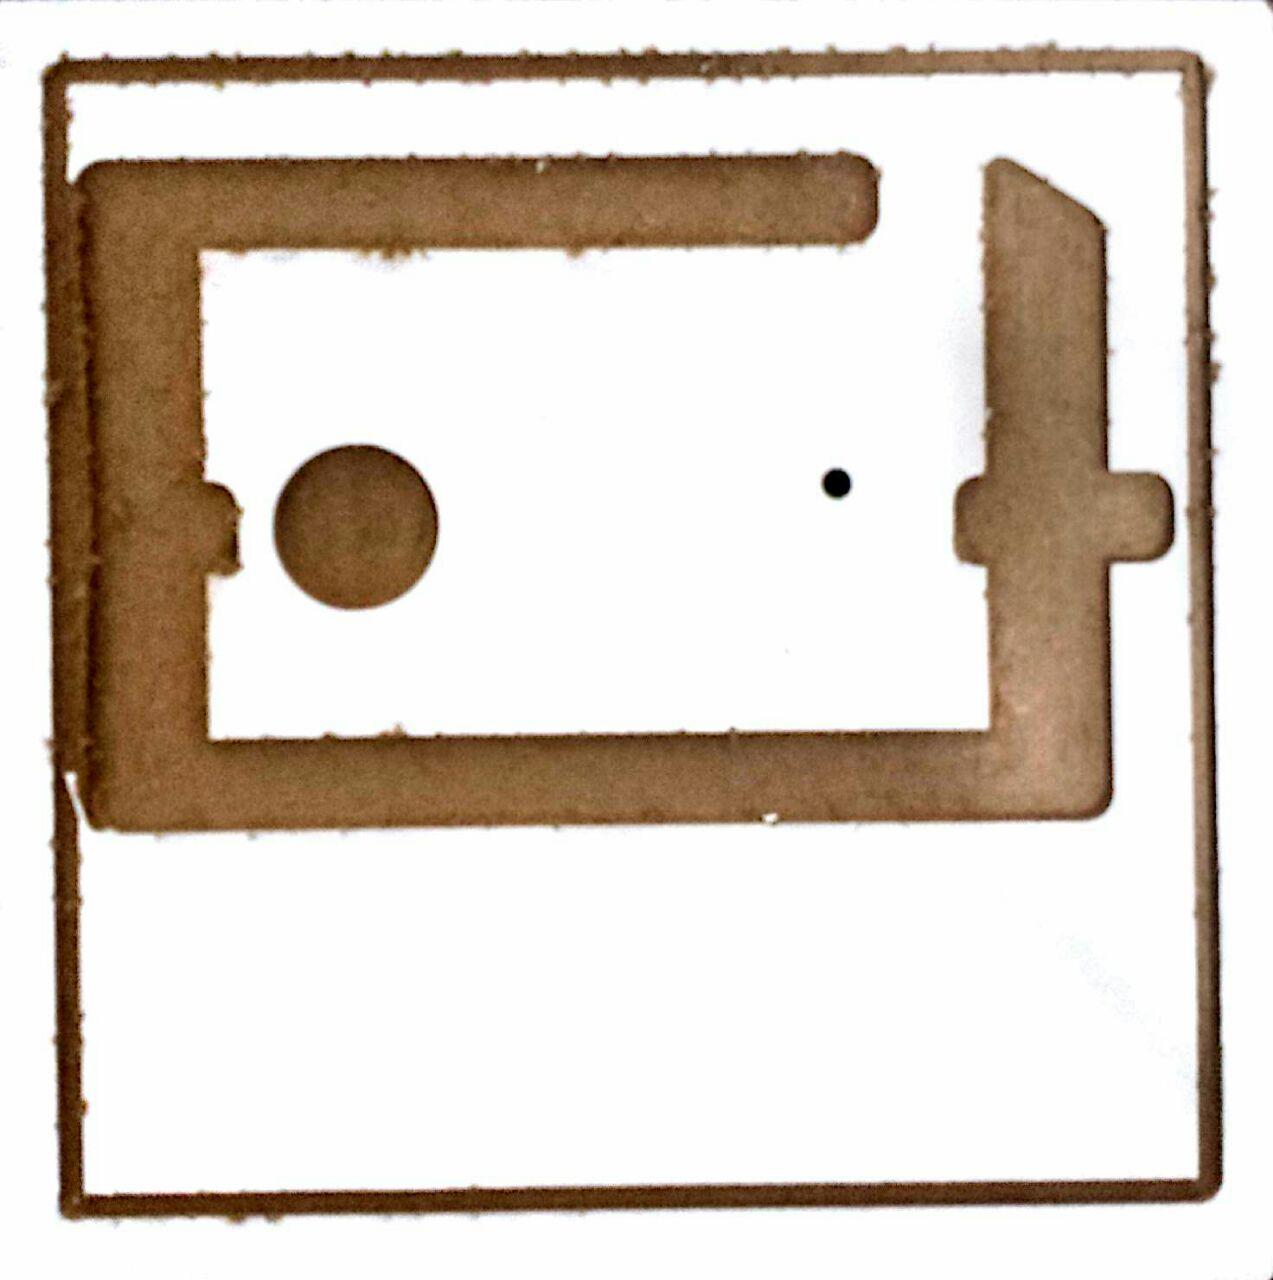
\includegraphics[width = 0.6\linewidth]{img/relat2/placaUsinada}
    \caption{Placa de Madeira Usinada com Defeito}
    \label{fig:placa-final}
\end{figure}

\subsection{Métrica do Desenho}
Para avaliar a qualidade de cada operação foram feitas diversas medidas da moldura desenhada em diferentes posições na largura e ao longo de seu comprimento e em comparadas com os valores iniciais de projeto.

\begin{table}[H]
    \centering
    \begin{tabular}{cccc}
    \hline
        & & \multicolumn{2}{c}{Peça}\\
        Posição & Projeto & Média & Variância\\
    \hline
         Bordas Horizontais & 175 & 174.93 & 0.63\\
         Bordas Verticais & 175 & 174.78 & 0.93\\
    \hline
    \end{tabular}
    \caption{Medidas da Peça}
    \label{tab:my_label}
\end{table}

\section{Discussão}

\section{Conclusão}
O código utilizado não foi capaz de concluir o desenho e no lugar acabou deixando um profundo furo na parte restante, além do desenho ter se misturado a borda deixando um aspecto ruim a qualidade final do trabalho. Para uma implementação futura do mesmo desenho é recomendado a utilização de uma escala menor bem com a descrição direta das coordenadas sem o uso de funções auxiliares como a $G92$ aplicadas na mudança de coordenadas no eixo $Z$ afinal ambos erros ocorridos se devem a valores inadequados nesta dimensão. O primeiro, na falha do perfilamento foi um erro para mais e o segundo no uso indevido da função $G92$ foi um erro para um valor muito inferior a espessura da placa.


% Prototipagem Rápida


% Referências ----------------------------------------------------------------------------------------------------------------------

\bibliographystyle{plain}
\bibliography{reference}


% Magno Correa
% http://buscatextual.cnpq.br/buscatextual/visualizacv.do?id=K4734325E3
% https://prezi.com/user/j4f46ctrnc3o/

% https://en.wikipedia.org/wiki/LinuxCNC

% ----------------------------------------------------------------------------------------------------------------------------------
\end{document}
